\documentclass[11pt]{article}
\usepackage[a4paper,margin=1in]{geometry}
\usepackage[T1]{fontenc}
\usepackage[utf8]{inputenc}
\usepackage{lmodern}
\usepackage{graphicx}
\usepackage{float}
\usepackage{booktabs}
\usepackage{listings}
\usepackage{hyperref}

\lstset{
  basicstyle=\ttfamily\small,
  breaklines=true,
  frame=single
}

\title{CircleNet Project Report (Task 2 and Task 3)}
\author{DS503 BDM}
\date{\today}

\begin{document}
\maketitle

\section{Scope}
This report covers:
\begin{itemize}
  \item \textbf{Task 2}: loading generated CSV datasets into HDFS.
  \item \textbf{Task 3}: analytics jobs (Task A to Task H) with simple and optimized approaches.
\end{itemize}
Dataset generation (Task 1) will be added later.

\section{Task 2: Loading Data into HDFS}
We used three CSV files:
\begin{itemize}
  \item CircleNetPage.csv
  \item Follows.csv
  \item ActivityLog.csv
\end{itemize}

Main HDFS commands used:
\begin{lstlisting}[language=bash]
hdfs dfs -mkdir /circlenet
hdfs dfs -mkdir /circlenet/pages
hdfs dfs -mkdir /circlenet/follows
hdfs dfs -mkdir /circlenet/activitylog

hdfs dfs -put data/CircleNetPage.csv /circlenet/pages/
hdfs dfs -put data/Follows.csv /circlenet/follows/
hdfs dfs -put data/ActivityLog.csv /circlenet/activitylog/
\end{lstlisting}

\begin{figure}[H]
  \centering
  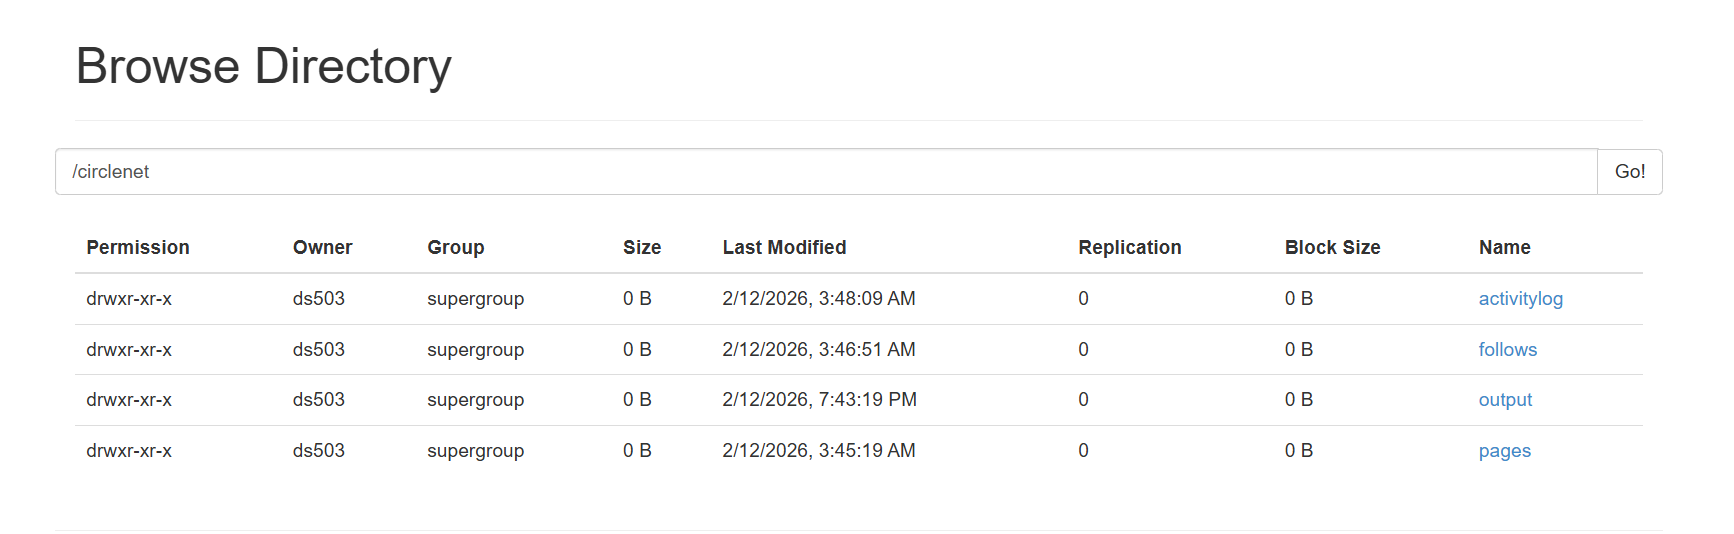
\includegraphics[width=0.9\textwidth]{screenshots_report/task2_data_loading_hdfs_1.png}
  \caption{HDFS folder creation and dataset loading}
\end{figure}

\begin{figure}[H]
  \centering
  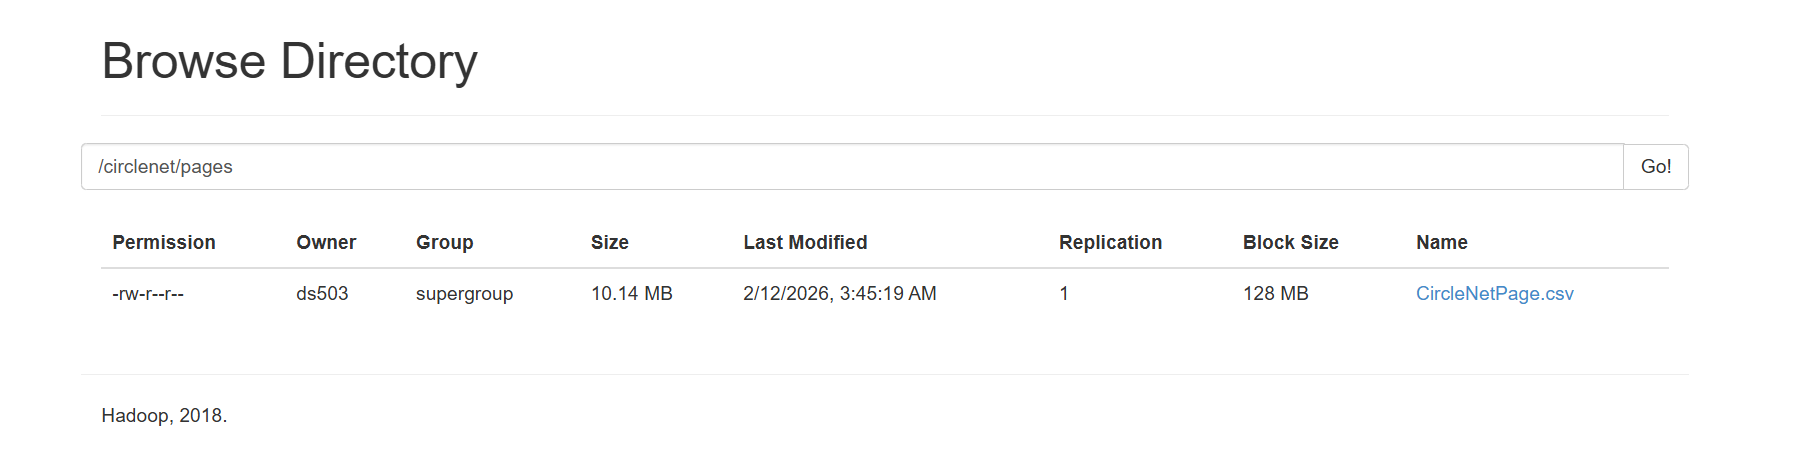
\includegraphics[width=0.8\textwidth]{screenshots_report/task2_pages_csv.png}
  \caption{CircleNetPage CSV sample}
\end{figure}

\begin{figure}[H]
  \centering
  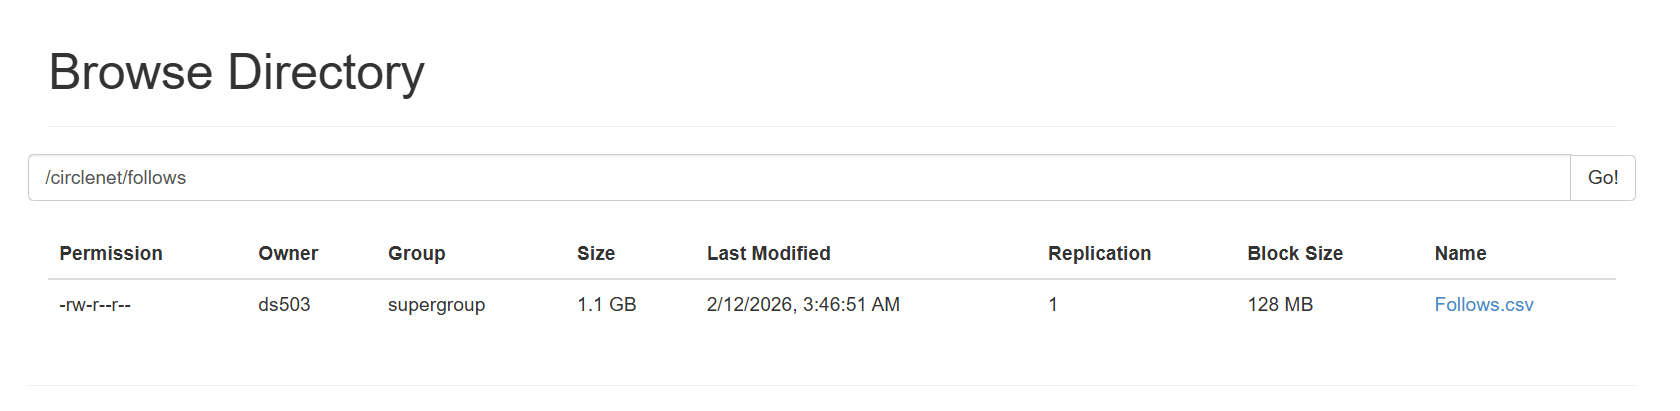
\includegraphics[width=0.8\textwidth]{screenshots_report/task2_follows_csv.png}
  \caption{Follows CSV sample}
\end{figure}

\begin{figure}[H]
  \centering
  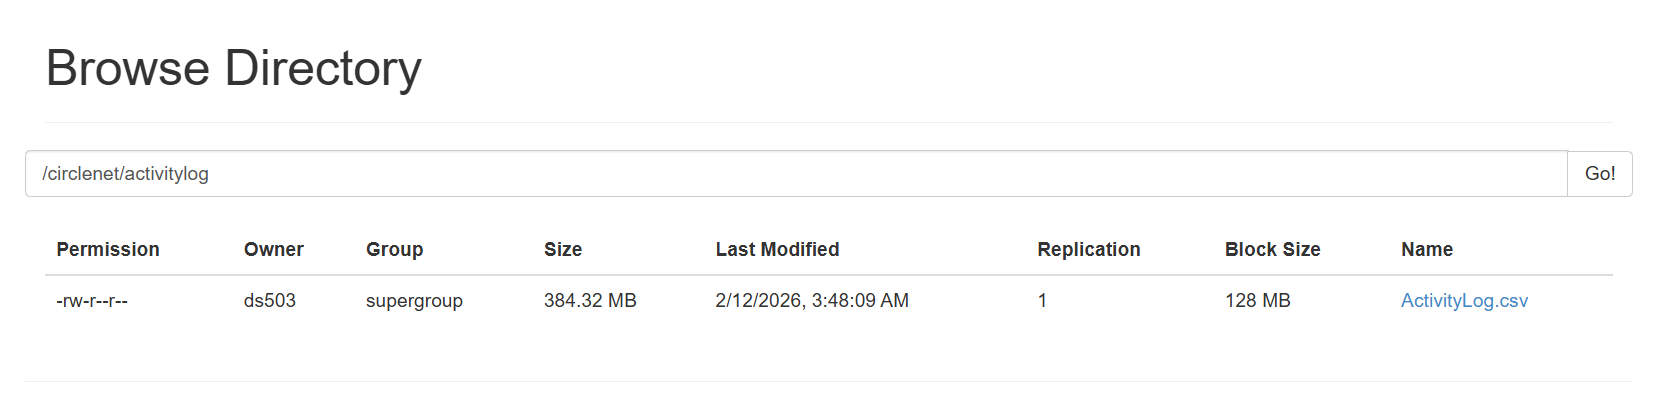
\includegraphics[width=0.8\textwidth]{screenshots_report/task2_activity_log_csv.png}
  \caption{ActivityLog CSV sample}
\end{figure}

\section{Task 3: Analytics Jobs (A--H)}
\subsection*{Execution and Timing Method}
Each job prints timing in milliseconds and also appends it to \texttt{task\_times.csv}. We used \texttt{phase=total} rows for final comparison.

\begin{lstlisting}[language=Java]
boolean ok = JobTimer.run(job, "TaskAOptimized");
JobTimer.total("TaskAOptimized", totalStart);
\end{lstlisting}

\subsection*{Task A: Hobby frequency}
\textbf{Jobs used:} Map-only jobs: 0, MapReduce jobs: 1.\\
\textbf{Simple solution:} We read CircleNetPage and emitted \texttt{(FavoriteHobby,1)} from mapper, then summed in reducer to get frequency per hobby. This directly matches the requirement and is easy to verify.\\
\textbf{Optimization:} We kept the same single-job structure and added a combiner because this operation is sum-only and safe for local aggregation. \textit{Optimized file:} \texttt{src/main/java/circlenet/taskA/TaskAOptimized.java}.\\
\textbf{Assumption:} hobby text values are already clean categorical values in input.\\
\textbf{Scalable aspect:} key-based partitioning distributes hobby groups across reducers and combiner lowers shuffle volume.
\textbf{Final output file used in report:} \texttt{output\_all/taskA/optimized/part-r-00000}
\textbf{Output shown below:} full output (all hobbies and their frequencies).
\begin{lstlisting}
BoardGameNights    5926
BubbleWrapPopping  2919
CheeseCollecting   1966
CloudWatching      2997
CoffeeHoarding     4913
CompetitiveGoogling 3018
Cooking            9916
EscapeRooming      3964
ExtremeCouponing   1977
Gaming             17822
Gardening          4811
Hiking             9017
MemeArcheology     5898
Music              11674
NappingCompetitively 4008
Painting           4928
PeopleWatching     4981
Photography        7834
PlantParenting     5900
PodcastBinging     6996
ProcrastinationArts 7963
Reading            11840
RetroGaming        4916
SockPuppetry       2018
Sports             13605
ThriftFlipping     3915
TrainSpotting      1863
Traveling          13753
UrbanExploring     2957
VinylHunting       2997
Writing            5778
Yoga               6930
\end{lstlisting}
\textbf{How to read output:} column 1 = hobby name, column 2 = frequency count. This exactly matches Task A.

\begin{figure}[H]
  \centering
  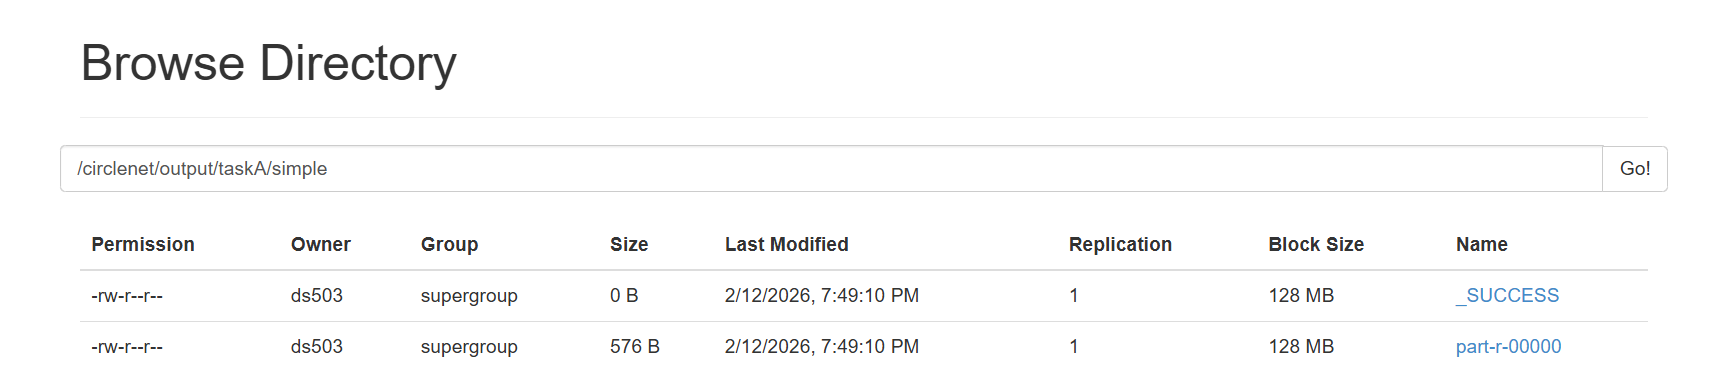
\includegraphics[width=0.82\textwidth]{screenshots_report/taskA_output_hdfs_simple.png}
  \caption{Task A simple output}
\end{figure}

\begin{figure}[H]
  \centering
  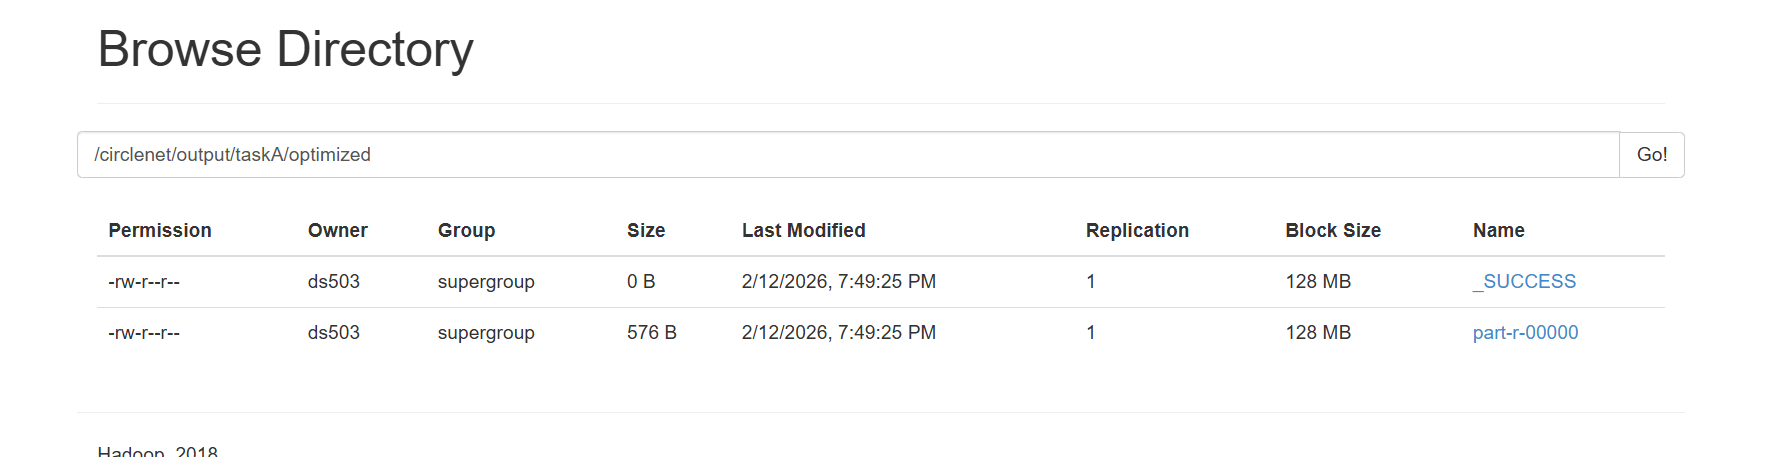
\includegraphics[width=0.82\textwidth]{screenshots_report/taskA_output_hdfs_optimized.png}
  \caption{Task A optimized output}
\end{figure}

\subsection*{Task B: Top 10 most accessed pages}
\textbf{Jobs used:} Simple: Map-only jobs: 0, MapReduce jobs: 3. Optimized: Map-only jobs: 0, MapReduce jobs: 2.\\
\textbf{Simple solution:} Job 1 counts accesses per page from ActivityLog. Job 2 combines those counts with page information to get \texttt{ID, NickName, JobTitle, Count}. Job 3 computes global top 10. This step-by-step pipeline is easy to reason about.\\
\textbf{Optimization:} We reduced pipeline depth by keeping counting as one stage (with combiner) and doing final top-10 output in a lighter second stage. \textit{Optimized file:} \texttt{src/main/java/circlenet/taskB/TaskBOptimized.java}.\\
\textbf{Assumption:} if multiple pages have equal access count, any deterministic order among ties is acceptable.\\
\textbf{Scalable aspect:} page-level counting is fully parallel by key; reducing one heavy stage lowers total shuffle/IO.
\textbf{Final output file used in report:} \texttt{output\_all/taskB/optimized/part-r-00000}
\textbf{Output shown below:} full output (all 10 rows).
\begin{lstlisting}
199507,Capybara913,Platform Consultant,82
21536,FalafelQueen,Regional Frontend Co,82
47445,ChurroPixel,Senior Data Analyst,82
104631,SnoringFerret,Assistant Coordinato,81
143770,KingPenguin,Nap Herder,81
144195,BouncingMeerkat,Assistant Security C,81
98996,AgentPlatypus,Staff Systems Resear,81
54560,TofuVolcano,Associate Product De,80
112890,ChurroSpoon,Marketing Designer,79
141449,RunningHedgehog,Legendary Emoji Wiza,79
\end{lstlisting}
\textbf{How to read output:} column 1 = ID, column 2 = NickName, column 3 = JobTitle, column 4 = access count used only as ranking evidence. Task B required ID, NickName, JobTitle; those are provided in columns 1--3.

\subsection*{Task C: Same hobby as selected hobby}
\textbf{Jobs used (final):} Map-only jobs: 1, MapReduce jobs: 0.\\
\textbf{Simple solution:} We filter CircleNetPage rows by one selected hobby and output \texttt{NickName, JobTitle} for matching users. Since this is only filtering/projection, the implementation stays simple and readable.\\
\textbf{Why no further optimization:} There is no aggregation, no ranking, and no join in the final requirement. Adding reducers or extra stages would only add overhead without improving output quality.\\
\textbf{Assumption:} selected hobby value is passed as input argument (for our run, one valid hobby string was used).\\
\textbf{Scalable aspect:} each mapper processes independent input splits; the task scales naturally with data partitions.
\textbf{Final output file used in report:} \texttt{output\_all/taskC/simple/part-r-00000}
\textbf{Output shown below:} excerpt only (full matching list is in the output file).
\begin{lstlisting}
AdmiralArmadillo    Chief Mobile Consult
AdmiralArmadillo    Frontend Engineer
AdmiralAxolotl      Data Designer
\end{lstlisting}
\textbf{How to read output:} column 1 = NickName, column 2 = JobTitle. This exactly matches Task C.

\subsection*{Task D: Popularity factor (followers per owner)}
\textbf{Jobs used:} Simple: Map-only jobs: 0, MapReduce jobs: 1. Optimized: Map-only jobs: 1, MapReduce jobs: 1.\\
\textbf{Simple solution:} We combine page owners and follows by owner ID and compute follower count. We also ensure owners with no followers are returned with zero so output is complete.\\
\textbf{Optimization:} We first aggregate follower counts as a dedicated stage (with safe count combiner), then run a lighter final stage for owner output formatting. \textit{Optimized file:} \texttt{src/main/java/circlenet/taskD/TaskDOptimized.java}.\\
\textbf{Assumption:} one follow edge contributes exactly one count to ID2 owner; duplicate lines are counted as separate relations if present in data.\\
\textbf{Scalable aspect:} follower aggregation is key-grouped and parallelized; this keeps large follow edges distributed.
\textbf{Final output file used in report:} \texttt{output\_all/taskD/optimized/part-m-00000}
\textbf{Output shown below:} excerpt only (full output has one row per page owner).
\begin{lstlisting}
1,FluffyHedgehog,199999
2,LordPlatypus,199999
3,FunkyHedgehog,199999
\end{lstlisting}
\textbf{How to read output:} column 1 = owner ID (extra identifier), column 2 = owner NickName, column 3 = follower count (popularity factor). Task D asked for nickname and follower count; both are present.

\subsection*{Task E: Favorites behavior}
\textbf{Requirement}: for each page owner, output total actions and number of distinct pages accessed.\\
\textbf{Important fix}: include owners with zero actions.\\
\textbf{Jobs used (final):} Map-only jobs: 0, MapReduce jobs: 1.\\
\textbf{Simple solution:} We join owner IDs with activity by owner key, then compute two values per owner: total actions and distinct pages accessed. Owners with no activity are explicitly included with \texttt{0,0}, so the result is correct for all owners.\\
\textbf{Why no further optimization:} Exact distinct counting per owner is the main cost here. Extra stages or extra reducers did not improve total runtime on our setup, so we kept the clean one-job version.\\
\textbf{Assumption:} output format is \texttt{ID <tab> totalActions,distinctPages}.\\
\textbf{Scalable aspect:} computation is partitioned by owner ID and remains distributed even with exact distinct counting.
\textbf{Final output file used in report:} \texttt{output\_all/taskE/simple/part-r-00000}
\textbf{Output shown below:} excerpt only (full output has one row per page owner ID).
\begin{lstlisting}
1    39,39
2    58,58
3    51,51
\end{lstlisting}
\textbf{How to read output:} left side = owner ID, right side = \texttt{totalActions,distinctPages}. This matches Task E (ID is enough, names not required).

\subsection*{Task F: More popular than average}
\textbf{Jobs used:} Simple: Map-only jobs: 0, MapReduce jobs: 3. Optimized: Map-only jobs: 0, MapReduce jobs: 2.\\
\textbf{Simple solution:} We compute follower count per owner, calculate global average follower count, and then filter owners above average. Multi-stage flow keeps each stage clear and testable.\\
\textbf{Optimization:} We use combiner in follower counting stage and reduce the heavy part of the pipeline before final filtering. \textit{Optimized file:} \texttt{src/main/java/circlenet/taskF/TaskFOptimized.java}.\\
\textbf{Assumption:} average is computed over all owners (including owners with zero followers).\\
\textbf{Scalable aspect:} the large counting stage is distributed by owner key, and reduced intermediate size helps overall throughput.
\textbf{Final output file used in report:} \texttt{output\_all/taskF/optimized/part-r-00000}
\textbf{Output shown below:} excerpt only (full output file contains all above-average owners).
\begin{lstlisting}
2797,SpinningShrimp,103
2779,HazyFerret,103
2771,MegaChinchilla,103
\end{lstlisting}
\textbf{How to read output:} column 1 = owner ID, column 2 = NickName, column 3 = follower count. Every row satisfies ``more followers than average'', which is exactly Task F.

\subsection*{Task G: Outdated users (no activity in last 90 days)}
\textbf{Jobs used:} Simple: Map-only jobs: 0, MapReduce jobs: 3. Optimized: Map-only jobs: 1, MapReduce jobs: 1.\\
\textbf{Simple solution:} First we compute latest global activity time, then each user's latest time, then filter users whose last activity is older than 90 days. This directly follows the problem statement.\\
\textbf{Optimization:} We reduce one stage and keep combiner only for \texttt{max} aggregation (safe operation). \textit{Optimized file:} \texttt{src/main/java/circlenet/taskG/TaskGOptimized.java}.\\
\textbf{Assumption:} ActionTime granularity is hour, so 90 days is treated as 2160 time units.\\
\textbf{Scalable aspect:} user-wise max aggregation is parallel by key and stage reduction lowers total IO.
\textbf{Final output file used in report:} \texttt{output\_all/taskG/optimized/part-m-00000}
\textbf{Output shown below:} excerpt only (full output file contains all outdated users).
\begin{lstlisting}
1,FluffyHedgehog
2,LordPlatypus
3,FunkyHedgehog
\end{lstlisting}
\textbf{How to read output:} column 1 = ID, column 2 = NickName. Each row is a page owner with no recent access in the last 90 days. This matches Task G.

\subsection*{Task H: Same region one-way follows}
\textbf{Jobs used:} Simple: Map-only jobs: 0, MapReduce jobs: 2. Optimized: Map-only jobs: 0, MapReduce jobs: 1.\\
\textbf{Simple solution:} We first identify one-way same-region follow relations, then in a second stage produce final user output fields. This keeps relation logic and output formatting separate.\\
\textbf{Optimization:} We combine this into one MapReduce stage while preserving the same one-way relation condition. \textit{Optimized file:} \texttt{src/main/java/circlenet/taskH/TaskHOptimized.java}.\\
\textbf{Assumption:} relationship is directional; \texttt{A->B} and \texttt{B->A} are different and must both exist to be considered mutual.\\
\textbf{Scalable aspect:} relation checks are key-grouped and the single-stage pipeline lowers repeated read/write overhead.
\textbf{Final output file used in report:} \texttt{output\_all/taskH/optimized/part-r-00000}
\textbf{Output shown below:} excerpt only (full output file contains all matching users).
\begin{lstlisting}
100,PretzelSpoon
1000,GeneralPenguin
10000,EpicMoose997
\end{lstlisting}
\textbf{How to read output:} column 1 = ID, column 2 = NickName. Each row is a person who follows someone in same region but is not followed back, which is exactly Task H.

\section{Performance Summary (from task\_times.csv)}
\begin{table}[H]
\centering
\begin{tabular}{lrrl}
\toprule
Task & Simple (ms) & Optimized (ms) & Final \\
\midrule
A & 3077 & 2048 & Optimized \\
B & 26156 & 18962 & Optimized \\
C & 2048 & -- & Simple (no further optimization needed) \\
D & 32764 & 22769 & Optimized \\
E & 24681 & -- & Simple (no further optimization needed) \\
F & 31431 & 23094 & Optimized \\
G & 35888 & 18015 & Optimized \\
H & 33018 & 26301 & Optimized \\
\bottomrule
\end{tabular}
\caption{Simple vs optimized total times (\texttt{phase=total})}
\end{table}

\section{Combiner Usage Decision}
\begin{itemize}
  \item Used where mathematically safe: sum/max aggregation tasks.
  \item Not forced where not useful or risky for correctness.
  \item For map-only logic, reducer/combiner is skipped.
\end{itemize}

\section{Conclusion}
We implemented solid simple solutions for all tasks and optimized only where it gives clear practical value. For Task C and Task E, the simple logic is final because further optimization is not needed and would add complexity without meaningful benefit.

\end{document}

